\documentclass{article}
\usepackage[utf8]{inputenc}
\usepackage[T2A]{fontenc}
\usepackage[russian]{babel} 


\usepackage{graphicx,amssymb,amsmath,amsfonts,latexsym,mathtext, mathrsfs, amsthm}
\usepackage[a4paper,left=2cm, right=2cm, top=2cm, bottom=2cm, bindingoffset=1cm]{geometry}

\usepackage{enumerate}

\usepackage{chngcntr}
\counterwithin*{equation}{section}

\usepackage{floatflt}
\renewcommand{\vec}[1]{\boldsymbol{#1}}
%\usepackage{indentfirst}   

\newcommand{\ph}{\varphi}
\newcommand{\ep}{\varepsilon}

\renewcommand{\ge}{\geqslant}
\renewcommand{\le}{\leqslant}

\newcommand{\R}{\mathbb{R}}
\newcommand{\LC}{L^2_\mathbb{C}}
\newcommand{\Co}{\mathbb{C}}
\newcommand{\la}{\lambda}
\newcommand{\sla}{\sqrt{\lambda}}
\newcommand{\sm}{\sqrt{\mu_n}}
\newcommand{\conj}[1]{\overline{#1}}
\newcommand{\Obig}[1]{O\left(#1\right)}

\DeclareMathOperator{\AC}{AC}
\DeclareMathOperator{\SL}{SL}
\DeclareMathOperator{\Ima}{Im}
\DeclareMathOperator{\Rea}{Re}

% figbr = figure bracket
\newcommand{\figbr}[1]{
	\left\{
	#1
	\right\}
}

% summa
\newcommand{\summ}[3]{\sum\limits_{#1=#2}^{#3}}

% integral
\newcommand{\intup}[1]{\int\limits_{0}^{#1}}

% sequence 1-a, 2-n, 3-1
\newcommand{\seq}[3]{\{{#1}_{#2}\}_{#2=#3}^{\infty}}

% question = qstn
\newcounter{vopros}

\newcommand{\qstn}{\par\noindent\addtocounter{vopros}{1}%
	\fbox{\textbf{Вопрос \arabic{vopros}}} \\ \par\noindent}

\newcommand{\bilet}[1]{\newpage\noindent%
	\fbox{\textbf{Билет #1}} \par\noindent}

\newcounter{z-counter}[section]
\newcounter{th-counter}[vopros]
\newcounter{df-counter}[vopros]
\newcounter{lm-counter}[vopros]
\newcounter{col-counter}[vopros]

\newcommand{\z}{\par\noindent\addtocounter{z-counter}{1}%
	\textbf{Задача \arabic{z-counter}.} }
\newcommand{\theor}{\par\noindent\addtocounter{th-counter}{1}%
	\textbf{Теорема \arabic{th-counter}.} }
\newcommand{\df}{\par\noindent\addtocounter{df-counter}{1}%
	\textbf{Опр. \arabic{df-counter}.} }
\newcommand{\lm}{\par\noindent\addtocounter{lm-counter}{1}%
	\textbf{Лемма \arabic{lm-counter}.} }
\newcommand{\note}{\par\noindent%
	\textbf{Замечание.} }
\newcommand{\col}{\par\noindent\addtocounter{col-counter}{1}%
	\textbf{Следствие \arabic{col-counter}.} }

\newdimen\theoremskip
\theoremskip=2pt
\renewenvironment{proof}{\par\noindent$\square\quad$}{$\hfill\blacksquare$ \par\vskip\theoremskip} %hfill for align at the end of line

\begin{document}

\Large\textbf{Тестовое задание в Ритм}

\section{Постановка исходной задачи}

\begin{align*}
    &\frac{d^5y}{dx^5} + 15\frac{d^4y}{dx^4} + 90\frac{d^3y}{dx^3} + 270\frac{d^3y}{dx^3} + 405\frac{d^y}{dx} + 243y = 0, \qquad x \in [0,5] \\
    &y\bigg|_{x=0} = 0, \quad \frac{dy}{dx}\bigg|_{x=0} = 3, \quad \frac{d^2y}{dx^2}\bigg|_{x=0} = -9, \quad \frac{d^3y}{dx^3}\bigg|_{x=0} = -8, \quad \frac{d^4y}{dx^4}\bigg|_{x=0} = 0
\end{align*}

\section{Решение}

Сведем уравнение 5-го порядка к системе первого порядка:

сделаем замену
\begin{align*}
    &y_1 = y\\
    &y_2 = y'\\
    &y_3 = y''\\
    &y_4 = y'''\\
    &y_5 = y^{(4)}\\
\end{align*}
получим систему
$$\begin{cases}
    y_1' = y_2\\
    y_2' = y_3\\
    y_3' = y_4\\
    y_4' = y_5\\
    y_5' = -243y_1 - 405y_2 - 270y_3 - 90y_4 - 15y_5\\
\end{cases}$$

Если ввести обозначение $y = (y_1, y_2, y_3, y_4, y_5)^T$, то можно переписать эту систему в матричном виде
$$y' = f(y) \equiv My,$$
где $M$ --- матрица 5х5:
$$ M = 
\begin{pmatrix}
    0 & 1 & 0 & 0 & 0\\
    0 & 0 & 1 & 0 & 0\\
    0 & 0 & 0 & 1 & 0\\
    0 & 0 & 0 & 0 & 1\\
    -243 & -405 & -270 & -90 & -15
\end{pmatrix}
$$

Воспользуемся модифицированном методе Эйлера решения задачи Коши, основанном на формуле трапеций
$$
\begin{cases}
    y^*=y_n + h f(y_n) = y_n + h My_n\\
    y_{n+1} = y_n + \frac{h}{2} (f(y_n) + f(y^*)) = y_n + \frac{h}{2} M(y_n + y^*)
\end{cases}
$$
Здесь $h$ --- это шаг по отрезку. Ошибка на отрезке в данном методе составляет $O(h^2)$, что лучше обычного метода Эйлера, который дает ошибку $O(h)$. Существуют методы Рунге-Кутта, которые могут дать более высокий порядок точности.

Таким образом, используя приведенный алгоритм, имея заданное начальное условие
$$y_0 = 
\begin{pmatrix}
    0\\
    3\\
    -9\\
    -8\\
    0
\end{pmatrix}
$$
можно найти приближенное значение первых пяти производных на разбиении отрезка. Но нам нужна сама функция, поэтому мы в конце концов оставим только значения исходной функции. 

Доказательство того, что эта функция действительно будет приближать решение, следует из формулы Тейлора.

\newpage
\section{График полученной функции}
\
\begin{figure}[h]
    \centering
	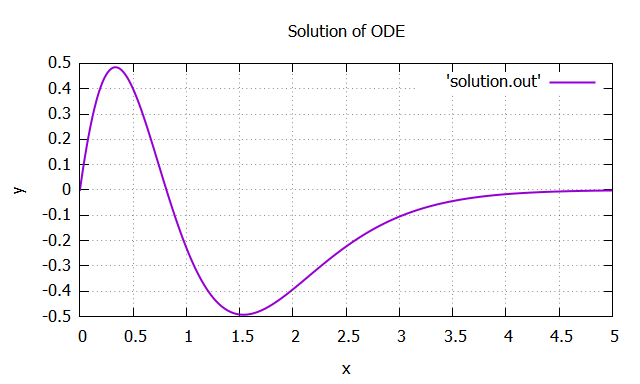
\includegraphics[width = 7cm]{result.png}
	\caption{$N = 1000$}
\end{figure}

\end{document}
